% !TeX spellcheck = russian-aot-ieyo
% Зачем: Определяет класс документа (То, как будет выглядеть документ)
% Примечание: параметр draft помечает строки, вышедшие за границы страницы, прямоугольником, в фильной версии его нужно удалить.
\documentclass[a4paper,14pt,russian,oneside,final]{extreport}

% Зачем: Настройка Times New Roman.
% Рекомендовано для Windows (нужен PSCyr, подробности см. в fonts_windows.tex)
% раскомментировать, чтобы использовать:
%\input{fonts_windows}% не забудьте закомментировать \input{fonts_linux}

% Рекомендовано для Linux (нужен scalable-cyrfonts-tex, подробности см. в fonts_linux.tex)
% раскомментировать, чтобы использовать:
\input{fonts_linux}% не забудьте закомментировать \input{fonts_windows}

% Зачем: Установка кодировки исходных файлов.
\usepackage[utf8]{inputenc}

% Зачем: Делает результирующий PDF "searchable and copyable".
\usepackage{cmap}

% Зачем: Чтобы можно было использовать русские буквы в формулах, но в случае использования предупреждать об этом.
\usepackage[warn]{mathtext}

% Зачем: Учет особенностей различных языков.
\usepackage[russian,english]{babel}

% Зачем: Добавляет поддержу дополнительных размеров текста 8pt, 9pt, 10pt, 11pt, 12pt, 14pt, 17pt, and 20pt.
% Почему: Пункт 2.1.1 Требований по оформлению пояснительной записки.
\usepackage{extsizes}


% Зачем: Длинна, пимерно соответвующая 5 символам
% Почему: Требования содержат странное требование про отсупы в 5 символов (для немоноширинного шрифта :| )
\newlength{\fivecharsapprox}
\setlength{\fivecharsapprox}{6ex}


% Зачем: Добавляет отступы для абзацев.
% Почему: Пункт 2.1.3 Требований по оформлению пояснительной записки.
\usepackage{indentfirst}
\setlength{\parindent}{\fivecharsapprox} % Примерно соответсвует 5 символам.


% Зачем: Настраивает отступы от границ страницы.
% Почему: Пункт 2.1.2 Требований по оформлению пояснительной записки.
\usepackage[left=3cm,top=2.0cm,right=1.5cm,bottom=2.7cm]{geometry}


% Зачем: Настраивает межстрочный интервал, для размещения 40 +/- 3 строки текста на странице.
% Почему: Пункт 2.1.1 Требований по оформлению пояснительной записки.
\usepackage[nodisplayskipstretch]{setspace}
\setstretch{1.1}
%\onehalfspacing

% Зачем: Выбор шрифта по-умолчанию.
% Почему: Пункт 2.1.1 Требований по оформлению пояснительной записки.
% Примечание: В требованиях не указан, какой именно шрифт использовать. По традиции используем TNR.
\renewcommand{\rmdefault}{ftm} % Times New Roman


% Зачем: Отключает использование изменяемых межсловных пробелов.
% Почему: Так не принято делать в текстах на русском языке.
\frenchspacing


% Зачем: Сброс счетчика сносок для каждой страницы
% Примечание: в "Требованиях по оформлению пояснительной записки" не указано, как нужно делать, но в других БГУИРовских докуметах рекомендуется нумерация отдельная для каждой страницы
\usepackage{perpage}
\MakePerPage{footnote}


% Зачем: Добавляет скобку 1) к номеру сноски
% Почему: Пункты 2.9.2 и 2.9.1 Требований по оформлению пояснительной записки.
\makeatletter
\def\@makefnmark{\hbox{\@textsuperscript{\normalfont\@thefnmark)}}}
\makeatother


% Зачем: Расположение сносок внизу страницы
% Почему: Пункт 2.9.2 Требований по оформлению пояснительной записки.
\usepackage[bottom]{footmisc}


% Зачем: Переопределяем стандартную нумерацию, т.к. в отчете будут только section и т.д. в терминологии TeX
\makeatletter
\renewcommand{\thesection}{\arabic{section}}
\makeatother


% Зачем: Пункты (в терминологии требований) в терминологии TeX subsubsection должны нумероваться
% Почему: Пункт 2.2.3 Требований по оформлению пояснительной записки.
\setcounter{secnumdepth}{3}


% Зачем: Настраивает отступ между таблицей с содержанимем и словом СОДЕРЖАНИЕ
% Почему: Пункт 2.2.7 Требований по оформлению пояснительной записки.
\usepackage{tocloft}
\setlength{\cftbeforetoctitleskip}{-1em}
\setlength{\cftaftertoctitleskip}{1em}


% Зачем: Определяет отступы слева для записей в таблице содержания.
% Почему: Пункт 2.2.7 Требований по оформлению пояснительной записки.
\makeatletter
\renewcommand{\l@section}{\@dottedtocline{1}{0.5em}{1.2em}}
\renewcommand{\l@subsection}{\@dottedtocline{2}{1.7em}{2.0em}}
\makeatother


% Зачем: Работа с колонтитулами
\usepackage{fancyhdr} % пакет для установки колонтитулов
\pagestyle{fancy} % смена стиля оформления страниц


% Зачем: Нумерация страниц располагается справа снизу страницы
% Почему: Пункт 2.2.8 Требований по оформлению пояснительной записки.
\fancyhf{} % очистка текущих значений
\fancyfoot[R]{\thepage} % установка верхнего колонтитула
\renewcommand{\footrulewidth}{0pt} % убрать разделительную линию внизу страницы
\renewcommand{\headrulewidth}{0pt} % убрать разделительную линию вверху страницы
\fancypagestyle{plain}{
    \fancyhf{}
    \rfoot{\thepage}}


% Зачем: Задает стиль заголовков раздела жирным шрифтом, прописными буквами, без точки в конце
% Почему: Пункты 2.1.1, 2.2.5, 2.2.6 и ПРИЛОЖЕНИЕ Л Требований по оформлению пояснительной записки.
\makeatletter
\renewcommand\section{%
  \clearpage\@startsection {section}{1}%
    {\fivecharsapprox}%
    {-1em \@plus -1ex \@minus -.2ex}%
    {1em \@plus .2ex}%
    {\raggedright\hyphenpenalty=10000\normalfont\large\bfseries\MakeUppercase}}
\makeatother


% Зачем: Задает стиль заголовков подразделов
% Почему: Пункты 2.1.1, 2.2.5 и ПРИЛОЖЕНИЕ Л Требований по оформлению пояснительной записки.
\makeatletter
\renewcommand\subsection{%
  \@startsection{subsection}{2}%
    {\fivecharsapprox}%
    {-1em \@plus -1ex \@minus -.2ex}%
    {1em \@plus .2ex}%
    {\raggedright\hyphenpenalty=10000\normalfont\normalsize\bfseries}}
\makeatother


% Зачем: Задает стиль заголовков пунктов
% Почему: Пункты 2.1.1, 2.2.5 и ПРИЛОЖЕНИЕ Л Требований по оформлению пояснительной записки.
\makeatletter
\renewcommand\subsubsection{
  \@startsection{subsubsection}{3}%
    {\fivecharsapprox}%
    {-1em \@plus -1ex \@minus -.2ex}%
    {\z@}%
    {\raggedright\hyphenpenalty=10000\normalfont\normalsize\bfseries}}
\makeatother

% Зачем: для оформления введения и заключения, они должны быть выровнены по центру.
% Почему: Пункты 1.1.15 и 1.1.11 Требований по оформлению пояснительной записки.
\makeatletter
\newcommand\sectioncentered{%
  \clearpage\@startsection {section}{1}%
    {\z@}%
    {-1em \@plus -1ex \@minus -.2ex}%
    {1em \@plus .2ex}%
    {\centering\hyphenpenalty=10000\normalfont\large\bfseries\MakeUppercase}%
    }
\makeatother



% Зачем: Задает стиль библиографии
% Почему: Пункт 2.8.6 Требований по оформлению пояснительной записки.
\bibliographystyle{styles/belarus-specific-utf8gost780u}


% Зачем: Пакет для вставки картинок
% Примечание: Объяснение, зачем final - http://tex.stackexchange.com/questions/11004/why-does-the-image-not-appear
\usepackage[final]{graphicx}
\DeclareGraphicsExtensions{.pdf,.png,.jpg,.eps}


% Зачем: Директория в которой будет происходить поиск картинок
\graphicspath{{figures/}}


% Зачем: Добавление подписей к рисункам
\usepackage[nooneline]{caption}
\usepackage{subcaption}

% Зачем: чтобы работала \No в новых латехах
\DeclareRobustCommand{\No}{\ifmmode{\nfss@text{\textnumero}}\else\textnumero\fi}

% Зачем: поворот ячеек таблиц на 90 градусов
\usepackage{rotating}
\DeclareRobustCommand{\povernut}[1]{\begin{sideways}{#1}\end{sideways}}


% Зачем: когда в формулах много кириллических символов команда \text{} занимает много места
\DeclareRobustCommand{\x}[1]{\text{#1}}


% Зачем: Задание подписей, разделителя и нумерации частей рисунков
% Почему: Пункт 2.5.5 Требований по оформлению пояснительной записки.
\DeclareCaptionLabelFormat{stbfigure}{Рисунок #2}
\DeclareCaptionLabelFormat{stbtable}{Таблица #2}
\DeclareCaptionLabelSeparator{stb}{~--~}
\captionsetup{labelsep=stb}
\captionsetup[figure]{labelformat=stbfigure,justification=centering}
\captionsetup[table]{labelformat=stbtable,justification=raggedright}
\renewcommand{\thesubfigure}{\asbuk{subfigure}}

% Зачем: Окружения для оформления формул
% Почему: Пункт 2.4.7 требований по оформлению пояснительной записки и специфические требования различных кафедр
% Пример использования смотри в course_content.tex, строка 5
\usepackage{calc}
\newlength{\lengthWordWhere}
\settowidth{\lengthWordWhere}{где}
\newenvironment{explanationx}
    {%
    %%% Следующие строки определяют специфические требования разных редакций стандартов. Раскоменнтируйте нужную строку
    %% стандартный абзац, СТП-01 2010
    %\begin{itemize}[leftmargin=0cm, itemindent=\parindent + \lengthWordWhere + \labelsep, labelsep=\labelsep]
    %% без отступа, СТП-01 2013
    \begin{itemize}[leftmargin=0cm, itemindent=\lengthWordWhere + \labelsep , labelsep=\labelsep]%
    \renewcommand\labelitemi{}%
    }
    {%
    %\\[\parsep]
    \end{itemize}
    }

% Старое окружение для "где". Сохранено для совместимости
\usepackage{tabularx}

\newenvironment{explanation}
    {
    %%% Следующие строки определяют специфические требования разных редакций стандартов. Раскоменнтируйте нужные 2 строки
    %% стандартный абзац, СТП-01 2010
    %\par
    %\tabularx{\textwidth-\fivecharsapprox}{@{}ll@{ --- } X }
    %% без отступа, СТП-01 2013
    \noindent
    \tabularx{\textwidth}{@{}ll@{ --- } X }
    }
    {
    \\[\parsep]
    \endtabularx
    }


% Зачем: Удобная вёрстка многострочных формул, масштабирующийся текст в формулах, формулы в рамках и др
\usepackage{amsmath}


% Зачем: Поддержка ажурного и готического шрифтов
\usepackage{amsfonts}


% Зачем: amsfonts + несколько сотен дополнительных математических символов
\usepackage{amssymb}


% Зачем: Окружения «теорема», «лемма»
\usepackage{amsthm}


% Зачем: Производить арифметические операции во время компиляции TeX файла
\usepackage{calc}

% Зачем: Производить арифметические операции во время компиляции TeX файла
\usepackage{fp}

% Зачем: Пакет для работы с перечислениями
\usepackage{enumitem}
\makeatletter
 \AddEnumerateCounter{\asbuk}{\@asbuk}{щ)}
\makeatother


% Зачем: Устанавливает символ начала простого перечисления
% Почему: Пункт 2.3.5 Требований по оформлению пояснительной записки.
\setlist{nolistsep}


% Зачем: Устанавливает символ начала именованного перечисления
% Почему: Пункт 2.3.8 Требований по оформлению пояснительной записки.
\renewcommand{\labelenumi}{\asbuk{enumi})}
\renewcommand{\labelenumii}{\arabic{enumii})}

% Зачем: Устанавливает отступ от границы документа до символа списка, чтобы этот отступ равнялся отступу параграфа
% Почему: Пункт 2.3.5 Требований по оформлению пояснительной записки.

\setlist[itemize,0]{itemindent=\parindent + 2.2ex,leftmargin=0ex,label=--}
\setlist[enumerate,1]{itemindent=\parindent + 2.7ex,leftmargin=0ex}
\setlist[enumerate,2]{itemindent=\parindent + \parindent - 2.7ex}

% Зачем: Включение номера раздела в номер формулы. Нумерация формул внутри раздела.
\AtBeginDocument{\numberwithin{equation}{section}}

% Зачем: Включение номера раздела в номер таблицы. Нумерация таблиц внутри раздела.
\AtBeginDocument{\numberwithin{table}{section}}

% Зачем: Включение номера раздела в номер рисунка. Нумерация рисунков внутри раздела.
\AtBeginDocument{\numberwithin{figure}{section}}


% Зачем: Дополнительные возможности в форматировании таблиц
\usepackage{makecell}
\usepackage{multirow}
\usepackage{array}


% Зачем: "Умная" запятая в математических формулах. В дробных числах не добавляет пробел
% Почему: В требованиях не нашел, но в русском языке для дробных чисел используется {,} а не {.}
\usepackage{icomma}

% Зачем: макрос для печати римских чисел
\makeatletter
\newcommand{\rmnum}[1]{\romannumeral #1}
\newcommand{\Rmnum}[1]{\expandafter\@slowromancap\romannumeral #1@}
\makeatother


% Зачем: Управление выводом чисел.
\usepackage{sistyle}
\SIdecimalsign{,}

% Зачем: inline-коментирование содержимого.
\newcommand{\ignore}[2]{\hspace{0in}#2}


% Зачем: Возможность коментировать большие участки документа
\usepackage{verbatim}


\usepackage{xcolor}


% Зачем: Оформление листингов кода
% Примечание: final нужен для переопределения режима draft, в котором листинги не выводятся в документ.
\usepackage[final]{listings}


% Зачем: настройка оформления листинга для языка F#
\definecolor{bluekeywords}{rgb}{0.13,0.13,1}
\definecolor{greencomments}{rgb}{0,0.5,0}
\definecolor{turqusnumbers}{rgb}{0.17,0.57,0.69}
\definecolor{redstrings}{rgb}{0.5,0,0}

\renewcommand{\lstlistingname}{Листинг}

\lstdefinelanguage{FSharp}
    {morekeywords={abstract,and,as,assert,base,begin,class,default,delegate,do,done,downcast,downto,elif,else,end,exception,extern,false,finally,for,fun,function,global,if,in,inherit,inline,interface,internal,lazy,let,let!,match,member,module,mutable,namespace,new,not,null,of,open,or,override,private,public,rec,return,return!,select,static,struct,then,to,true,try,type,upcast,use,use!,val,void,when,while,with,yield,yield!,asr,land,lor,lsl,lsr,lxor,mod,sig,atomic,break,checked,component,const,constraint,constructor,continue,eager,event,external,fixed,functor,include,method,mixin,object,parallel,process,protected,pure,sealed,tailcall,trait,virtual,volatile},
    keywordstyle=\bfseries\color{bluekeywords},
    sensitive=false,
    morecomment=[l][\color{greencomments}]{///},
    morecomment=[l][\color{greencomments}]{//},
    morecomment=[s][\color{greencomments}]{{(*}{*)}},
    morestring=[b]",
    stringstyle=\color{redstrings},
    }

\lstdefinestyle{fsharpstyle}{
   xleftmargin=0ex,
   language=FSharp,
   basicstyle=\footnotesize\ttfamily,
   breaklines=true,
   columns=fullflexible
}

\lstdefinestyle{csharpinlinestyle} {
  language=[Sharp]C,
  morekeywords={yield,var,get,set,from,select,partial,where,async,await},
  breaklines=true,
  columns=fullflexible,
  basicstyle=\footnotesize\ttfamily
}

\lstdefinestyle{csharpstyle}{
  language=[Sharp]C,
  frame=lr,
  rulecolor=\color{blue!80!black}}


% Зачем: Нумерация листингов в пределах секции
\AtBeginDocument{\numberwithin{lstlisting}{section}}

\usepackage[normalem]{ulem}

\usepackage[final,hidelinks]{hyperref}
% Моноширинный шрифт выглядит визуально больше, чем пропорциональный шрифт, если их размеры одинаковы. Искусственно уменьшаем размер ссылок.
\renewcommand{\UrlFont}{\small\rmfamily\tt}

\usepackage[square,numbers,sort&compress]{natbib}
\setlength{\bibsep}{0em}

% Магия для подсчета разнообразных объектов в документе
\usepackage{lastpage}
\usepackage{totcount}
\regtotcounter{section}

\usepackage{etoolbox}

\newcounter{totfigures}
\newcounter{tottables}
\newcounter{totreferences}
\newcounter{totequation}

\providecommand\totfig{}
\providecommand\tottab{}
\providecommand\totref{}
\providecommand\toteq{}

\makeatletter
\AtEndDocument{%
  \addtocounter{totfigures}{\value{figure}}%
  \addtocounter{tottables}{\value{table}}%
  \addtocounter{totequation}{\value{equation}}
  \immediate\write\@mainaux{%
    \string\gdef\string\totfig{\number\value{totfigures}}%
    \string\gdef\string\tottab{\number\value{tottables}}%
    \string\gdef\string\totref{\number\value{totreferences}}%
    \string\gdef\string\toteq{\number\value{totequation}}%
  }%
}
\makeatother

\pretocmd{\section}{\addtocounter{totfigures}{\value{figure}}\setcounter{figure}{0}}{}{}
\pretocmd{\section}{\addtocounter{tottables}{\value{table}}\setcounter{table}{0}}{}{}
\pretocmd{\section}{\addtocounter{totequation}{\value{equation}}\setcounter{equation}{0}}{}{}
\pretocmd{\bibitem}{\addtocounter{totreferences}{1}}{}{}



% Для оформления таблиц не влязящих на 1 страницу
\usepackage{longtable}

% Для включения pdf документов в результирующий файл
\usepackage{pdfpages}

% Для использования знака градуса и других знаков
% http://ctan.org/pkg/gensymb
\usepackage{gensymb}

% Зачем: преобразовывать текст в верхний регистр командой MakeTextUppercase
\usepackage{textcase}

% Зачем: Переносы в словах с тире.
% Тире в словае заменяем на \hyph: аппаратно\hyphпрограммный.
% https://stackoverflow.com/questions/2193307/how-to-get-latex-to-hyphenate-a-word-that-contains-a-dash#
\def\hyph{-\penalty0\hskip0pt\relax}

% Добавляем абзацный отступ для библиографии
% https://github.com/mstyura/bsuir-diploma-latex/issues/19
\setlength\bibindent{-1.0900cm}

\makeatletter
\renewcommand\NAT@bibsetnum[1]{\settowidth\labelwidth{\@biblabel{#1}}%
   \setlength{\leftmargin}{\bibindent}\addtolength{\leftmargin}{\dimexpr\labelwidth+\labelsep\relax}%
   \setlength{\itemindent}{-\bibindent+\fivecharsapprox-0.240cm}%
   \setlength{\listparindent}{\itemindent}
\setlength{\itemsep}{\bibsep}\setlength{\parsep}{\z@}%
   \ifNAT@openbib
     \addtolength{\leftmargin}{\bibindent}%
     \setlength{\itemindent}{-\bibindent}%
     \setlength{\listparindent}{\itemindent}%
     \setlength{\parsep}{10pt}%
   \fi
}

% Нумерованный список с арабскими цифрами на всех уровнях нумерации
\usepackage{enumitem}
\newlist{legal}{enumerate}{10}
\setlist[legal]{label*=\arabic*.}

% Генерация текста-заполнителя
\usepackage{blindtext}


\input{macro_glob}

\begin{document}

\begin{titlepage}
  \begin{center}
    Министерство образования Республики Беларусь \\[1em]
    Учреждение образования \\
    БЕЛОРУССКИЙ ГОСУДАРСТВЕННЫЙ УНИВЕРСИТЕТ \\
    ИНФОРМАТИКИ И РАДИОЭЛЕКТРОНИКИ \\[1em]

    Факультет компьютерных систем и сетей \\ [1em]
    Кафедра электронных вычислительных машин \\[2em]

    \begin{flushright}
      \begin{minipage}{0.4\textwidth}
        К ЗАЩИТЕ ДОПУСТИТЬ: \\
        Зав. каф. ЭВМ \\
        \underline{\hspace*{2.8cm}} Д.\,И.~Самаль
      \end{minipage}\\[2.2em]
    \end{flushright}

    %%
    %% ВНИМАНИЕ: на некторых факультетах (ФКП) и кафедрах (ПИКС) слова "ПОЯСНИТЕЛЬНАЯ ЗАПИСКА" предлагается (требуется) оформлять полужирным начертанием. Раскомментируйте нужную для вас строку:
    %%
    %\textbf{ПОЯСНИТЕЛЬНАЯ ЗАПИСКА}\\
    {ПОЯСНИТЕЛЬНАЯ ЗАПИСКА}\\
    {к дипломному проекту}\\
    {на тему}\\
    {СИСТЕМА ФУНКИЦОНАЛЬНОГО КОНТРОЛЯ ТЕХНИЧЕСКИХ СРЕДСТВ КОМПЛЕКСА МАШИН УПРАЛЕНИЯ АРИЛЛЕРИЙСКОГО ДИВИЗИОНА}\\[2em]


    {БГУИР ДП 1--400201 01 600 ПЗ}\\[2em]

    \begin{tabular}{ p{0.65\textwidth}p{0.25\textwidth} }
      Студент & А.\,В.~Стаховский\\[1em]
      Руководитель & Т.\,В.~Державская \\[1em]
      Консультанты: &\\[1em]
      \hspace*{3ex}от кафедры ЭВМ & С.\,А.~Байрак \\[1em]
      \hspace*{3ex}по экономической части & Т.\,Л.~Слюсарь \\[1em]
      %%
      %% ВНИМАНИЕ: в зависимости от выбранной темы, у вас консультант может быть как по охране труда, так и по:
        % экологической безопасности
        % ресурсосбережению
        % энергосбережению
      %%
      %% Впишите правильную формулировку по необходимости
      Нормоконтролер & А.\,С.~Сидорович\\[1em]
      Рецензент &
    \end{tabular}

    \vfill
    {\normalsize МИНСК 2018}
  \end{center}
\end{titlepage}
 % page 1

% \sectioncentered*{Задание}
\thispagestyle{empty}
%%
%% ВНИМАНИЕ: этот реферат не соответствует СТП-01 2013
%% пример оформления реферата смотрите здесь: http://www.bsuir.by/m/12_100229_1_91132.docx
%%

% \vspace{4\parsep}

\begin{flushleft}
    \textbf{Задание}: разработка микро-ЭВМ на ПЛИС.

    Характеристики:
\end{flushleft}

\begin{itemize}
\item Вариант: 13
\item Тип архитектуры: Принстонская
\item Разрядность шины адреса: 11
\item Разрядность шины данных: 16
\item ПЗУ: синхронное
\item ОЗУ: синхронное
\item Тип адресации: косвенная регистровая
\item Команда условного перехода: JS
\item РОН: 10 штук
\item КЭШ: k = 2, алгоритм замещения строк – наименьшего использования, синхронизация с памятью - простая отложенная
\item Арифметические команды: DEC
\item Логические команды: AND, NAND
\item Сдвиговые команды: ROR
\item Арбитраж шин: централизованный последовательный
\item Стек: 11/вверх
\item Схема предсказателя переходов: А4, 4 бита, PC xor GHR
\item КПДП
\end{itemize}

\clearpage
 % page 2
%
% {
    \newgeometry{top=1.25cm,bottom=1.25cm,right=1cm,left=2cm,twoside}
    \thispagestyle{empty}
    \setlength{\parindent}{0em}

    \newcommand{\lineunderscore}{\uline{\hspace*{\fill}}}

    \begin{center}
        Министерство образования Республики Беларусь\\[1em]
        Учреждение образования\\
        БЕЛОРУССКИЙ ГОСУДАРСТВЕННЫЙ УНИВЕРСИТЕТ \\
        ИНФОРМАТИКИ И РАДИОЭЛЕКТРОНИКИ\\[1em]
    \end{center}

    \begin{minipage}{\textwidth}
        \begin{flushleft}
            Факультет: КСиС. Кафедра: ЭВМ. \\
            Специальность: 40 02 01 ``Вычислительные машины, системы и сети''.
            Специализация: 400201-01 ``Проектирование и применение локальных компьютерных сетей''.
        \end{flushleft}
    \end{minipage}\\[1em]

    \begin{minipage}{\textwidth}
        \begin{flushright}
            \begin{tabular}{p{0.40\textwidth}}
                УТВЕРЖДАЮ \\
                Заведующий кафедрой ЭВМ \\
                \underline{\hspace*{5em}}Д.И.~Самаль \\
                <<\underline{\hspace*{4ex}}>>\underline{\hspace*{6em}}2018 г.
            \end{tabular}
        \end{flushright}
    \end{minipage}

    \begin{center}
        ЗАДАНИЕ \\
        по дипломному проекту студента \\
        Стаховского Антона Владимировича
    \end{center}

    \begin{flushleft}
        1. Тема проекта: <<Система функционального контроля комплекса машин управления артиллерийского дивизиона>> --
        утверждена приказом по университету от 25 января 2018 г. \No{177}-с

        \vspace{1em}

        2. Срок сдачи студентом законченного проекта: 1 июня 2018 г.

        \vspace{1em}

        3. Исходные данные к проекту:

        \vspace{1em}

        4. Содержание пояснительной записки (перечень подлежащих разработке вопросов):

        5. Перечень графического материала (с точным указанием обязательных чертежей):

        \vspace{1em}

        6. Содержание задания по экономической части:
        \lineunderscore\\
        \lineunderscore\\
        \lineunderscore

        Задание выдал: \hfill{} \uline{\hspace*{6em}} / Т.\,Л.~Слюсарь /

        \vspace{1em}

    \end{flushleft}

    Задание выдал:  \hfill{} \uline{\hspace*{6em}} / И.\,О.~Фамилия /

    \begin{center}
        КАЛЕНДАРНЫЙ ПЛАН
    \end{center}

    \begin{tabular}{
            | >{\centering}m{0.40\textwidth}
            | >{\centering}m{0.08\textwidth}
            | >{\centering}m{0.22\textwidth}
        | >{\centering\arraybackslash}m{0.16\textwidth}|}
        \hline Наименование этапов дипломного проекта (работы) & Объем этапа, \% & Срок выполнения этапов & Примечание \\
        \hline & & & \\
        \hline & & & \\
        \hline & & & \\
        \hline & & & \\
        \hline & & & \\
        \hline & & & \\
        \hline & & & \\
        \hline & & & \\
        \hline & & & \\
        \hline & & & \\
        \hline & & & \\
        \hline
    \end{tabular}

    Дата выдачи задания: 23 марта 2018 г.\\
    Руководитель \hfill{} \uline{\hspace*{4em}} / И.\,О.~Фамилия /

    Задание принял к исполнению \hfill{} \uline{\hspace*{4em}} / И.\,О.~Фамилия /

    \restoregeometry
}
 % pages 3 and 4. printed separately

% \input{annotation} % not part of report

%\input{feedback} % not part of report

%\input{review} % not part of report

% \setcounter{page}{5}
%
% \input{table_of_contents}
%
% \sectioncentered*{Введение}
\addcontentsline{toc}{section}{Введение}
\label{sec:intro}

Защита своих границ и граждан -- одна из наиболее приоритетных задач любого государства.
Страна, которая не уделяет достаточного внимания состоянию своих войск и вооружения не может гарантировать безопасность своих граждан и сохранениее дальнейшее сохранение суверенитета.

За последние десятилетия военная техника и вооружение ушли далеко вперед.
Стали широко применяться различные датчики, спутниковые системы навигации, компьютерные сети, портативные компьютеры.
Благодаря внедрению автоматизации в расчеты, настройку оборуования, тестирование переферийных устройств эффективность вооруженных сил значительно возрасла.
Во время эксплуатации военной техники внезапный отказ технических средств и локальной вычислительной сети может привести
к серьезным потерям личного состава, порче оборудования, потере преимущества на местности.
В таких условиях автоматизация процессов проведения тестирования является одной из наиболее приоритетных задач.

Исключительную важность во время проведения боевых действий представляет комплекс машин управления огнем, который служит для управления офицерским составом деятельностью своих подчиненных.

Целью данного дипломного проекта является разработка и реализация системы автоматизации процессов тестирования технических средств и каналов обмена данными в локальной сети.
Данная система в первую очередь ориентированна на использование артиллерийским дивизионом, но при небольших доработках программные модули могут быть также использованы в решениях для других армейских подразделений.

Для успешного выполнения поставленной цели, работа над проектом была разбита на следующие задачи:
\begin{itemize}
    \item выбор технологий, удовлетворяющих требованиям
    \item разработка системы функционального тестирования навигационной системы
    \item разработка системы функционального контроля средств связи
    \item разработка системы фукнкионального контроля локальной сети
    \item разработка системы настройки и тестирования метеокомплекта
\end{itemize}

Система состоит из нескольких модулей, каждый из которых тестирует определенное устройство.
Подключение к внешним устройствам осуществляется через интерфейс RS-232 либо через локальную сеть.
Взаимодействие между машинами может происходить как через локальную сеть, так и через радиоканал.
\clearpage


\section{Разработка общей структуры микро-ЭВМ}
\label{sec:domain}

В данном разделе приводится функциональный состав разрабатываемой микро-ЭВМ, разработка и описание системы команд, а также описание взаимодействия всех блоков при выполнении команд программы.
\subsection{Функциональный состав микро-ЭВМ}
\label{sub:domain:bayes_net}
Для правильной работы и выполнения операций микро-ЭВМ должна обладать определенным набором функциональных блоков. Этот набор определяется архитектурой разрабатываемой микро-ЭВМ и требованиями, которые предъявляются при проектировании. Опишем набор функциональных блоков микро-ЭВМ для нашего варианта.

Наша микро-ЭВМ состоит из семи основных блоков: устройство управления, блок выборки инструкций, блок выборки операндов, блок выполнения, блок регистров, блок записи результата, память.

Устройство управления выставляет сигналы, необходимые для начала работы других блоков, устанавливает максимальное количество тактов работы для каждого устройства.

Блок выборки инструкций осуществляет выборку и декодирование команд. Этот блок включает в себя блок выборки, блок декодирования. Блок выборки в свою очередь содержит программный счетчик, который указывает на текущую команду в памяти команд. Блок декодирования принимает из памяти команд очередную команду и осуществляет разделение команды на отдельные составляющие (код операции, адреса регистров, памяти и т.д.).

Блок выборки операндов осуществляет загрузку операндов из регистров или RAM.

Блок исполнения предназначен для исполнения команд, поступающих из блока выборки операндов.
Он содержит блоки: стек, арифметико-логическое устройство (АЛУ). АЛУ хранит регистр флагов, который используется при переходе JS.

Блок записи результата осуществляет запись данных в РОН или ОЗУ.

Память в нашей архитектуре разделяется на два модуля.
Первый модуль является памятью команд, который представляет собой синхронную ROM,
тактируемую процессором.
Второй предназначен для хранения данных, над которыми производятся операции.
Память данных является синхронной RAM, и её тактирование также осуществляется процессором.
Оба модуля имеют размер в 1024 слов по два байта, так как размер шины адреса по условию равен 11 бит, а старший бит определяет какому модулю принадлежит адрес. Это позволяет иметь общее адресное пространство для RAM и ROM, так как микро-ЭВМ построена на Принстонской архитектуре. Если старший бит -- 1, то младшие 10 бит -- адрес RAM, в противном случае -- это адрес ROM.

Блок РОН содержит 10 шестнадцатиразрядных регистров, доступ к которым осуществляется за один такт процессорного времени, что позволяет значительно ускорить время обработки данных. Стек содержит 11 шестнадцатиразрядных регистров, объединенных в структуру доступа LIFO (last in first out), что может пригодиться в некоторых операциях обработки данных. Шестнадцатиразрядное АЛУ предназначено для выполнения четырех различных операций, что является главной задачей процессора.

\subsection{Разработка системы команд}
Для того, чтобы процессор мог выполнять определенные действия, необходимые для правильной обработки данных, должен быть разработан четкий набор инструкций, с помощью которого можно записать алгоритм на понятном процессору языке. В таблице 1.1 приведены все команды и способы их кодирования, разработанные в соответствии с заданным вариантом.

Как видно из таблицы 1.1  разрабатываемая микро-ЭВМ «понимает» 16 команд, с помощью которых можно построить различные алгоритмы обработки данных.

Процессор спроектированной системы поддерживает следующие типы адресации в командах АЛУ:
\begin{itemize}
    \item Прямая – адресация, при которой адрес в памяти указывается непосредственно в команде.
    \item Косвенная регистровая – номер регистра, в котором хранится адрес ячейки памяти, указывается непосредственно в команде
\end{itemize}
Также присутствуют команды MOV, позволяющие пересылать данные между регистрами, регистром и памятью, и загружать данные в регистр непосредственно из операнда команды.

Операции PUSH, POP предназначены для работы со стеком и работают с регистрами.

Операции перехода позволяют совершать безусловные переходы и переходы по условию. Операция JS совершает переход в случае, если установлен флаг S (флаг знака, означает, что старший бит результата АЛУ равен 1).
Операция JMP осуществляет безусловный переход.

И, наконец, операция HLT завершает работу процессора, сбрасывает регистры КЭШ и останавливает тактирование.

\begin{table}[ht]
\caption{Список команд микро-ЭВМ}
\label{table:domain:learning:number_of_models}
\centering
  \begin{tabular}{| >{\centering}m{0.1\textwidth}
                  | >{\raggedright}m{0.22\textwidth}
                  | >{\centering}m{0.14\textwidth}
                  | >{\centering}m{0.14\textwidth}
                  | >{\centering}m{0.13\textwidth}
                  | >{\centering\arraybackslash}m{0.11\textwidth}|}
      \hline КОП & Мнемоническая запись команды & Бит[31-16] & Бит[15-12] & Бит[11-8] & Бит[7-4] \\
      \hline 0000 & DEC [reg] & -- & КОП & -- & [reg] \\
      \hline 0001 & AND reg, [reg] & -- & КОП & reg & [reg] \\
      \hline 0010 & NAND reg, [reg] & -- & КОП & reg & [reg] \\
      \hline 0011 & ROR reg, [reg] & -- & КОП & reg & [reg] \\
      \hline 0100 & MOV reg, \$mem & \$mem & КОП & reg & -- \\
      \hline 0101 & PUSH reg & -- & КОП & reg & --  \\
      \hline 0110 & JMP \$mem & \$mem & КОП & -- & -- \\
      \hline 0111 & MOV reg, [reg] & -- & КОП & reg & [reg] \\
      \hline 1000 & DEC reg & -- & КОП & reg & -- \\
      \hline 1001 & AND reg, reg & -- & КОП & reg & reg \\
      \hline 1010 & NAND reg, reg & -- & КОП & reg & reg \\
      \hline 1011 & ROR reg, reg & -- & КОП & reg & reg  \\
      \hline 1100 & MOV \$mem, reg & -- & КОП & reg & -- \\
      \hline 1101 & POP reg & -- & КОП & reg & -- \\
      \hline 1110 & JS \$mem & \$mem & КОП & -- & -- \\
      \hline 1111 & HLT & - & КОП & -- & -- \\
      \hline
  \end{tabular}
\end{table}

В таблице \$mem означает, адрес ячейки памяти. Первый операнд (биты[11-8]) всегда адрес регистра, второй -- адрес ячейки памяти, регистр, или регистр, служащий для косвенной адресвации.
Если второй операнд -- адрес ячейки памяти, то он хранится в старших битах второго слова.
Если он адрес регистра -- хранится в битах[7-4].

Все команды имеют длину в два слова, операнды могут отсутствовать.
Первое и второе слово дополняются нулями.
Расположение операндов не зависит от мнемоники.

\subsection{Описание взаимодействия всех блоков микро-ЭВМ при выполнении команд программы}
Запуск микро-ЭВМ происходит при подаче нулевого сигнала на вход запуска. При этом сигнал попадает в блок выборки блока операций. Блок выборки выставляет на шину адреса команд нулевой адрес РС, по которому расположена первая команда, и формирует сигнал запроса следующей команды из памяти команд.

Блок памяти команд воспринимает сигнал запроса команды и её адрес, выставляет содержимое ячейки памяти, формирует сигнал готовности команды, и отправляет информацию в блок декодирования.

Блок декодирования читает данные с шины данных команд, и, в зависимости от кода операции, сохраняет части прочитанной информации в регистры (например, заносит код операции и адреса операндов в соответствующие регистры). Информация в этих регистрах будет храниться вплоть до её отправки в блок исполнения. Но пока декодеру нужно решить, состоит ли прочитанная команда из одного или двух слов. Если команда состоит из двух слов, то декодер формирует сигнал запроса второго слова команды и отправляет в блок выборки. При этом блок выборки инкрементирует РС и формирует сигнал запроса команды из памяти команд.

Когда все слова операции выбраны и декодированы декодер формирует сигнал готовности блока операций. Это значит, что стадия вычитки и декодирования завершилась и нам нужно ожидать завершения работы блока исполнения (если он занят выполнением своей стадии конвейера).

Как только блок исполнения освобождается, регистры с информацией об операции из блока декодирования копируются в аналогичные регистры блока исполнения. Блок операции начинает вычитывать следующую операцию, а блок исполнения (а точнее устройство управления) устанавливает флаг своей занятости и принимается исполнять команду.

В соответствии с кодом пришедшей операции УУ подает управляющие сигналы на все исполняющие блоки (РОН, стек, АЛУ, кэш), а также «открывает/закрывает» необходимые шины.

Если производится операция над операндами из регистров или непосредственным операндом, то выполнение разбивается на 2 стадии по одному такту на каждую: отправка данных на АЛУ, и сохранение результатов в регистре. Если один из операндов берется из памяти, то подаются соответствующие сигналы на кэш и происходит чтение данных. Чтение данных может длиться разное количество тактов в зависимости от наличия данных в строке и от степени наполненности кэша. Поэтому выполнение таких операций завершается на следующий такт после выдачи кэшем данных.

После завершения работы блока исполнения происходит защелкивание флагов состояния процессора и освобождение флага занятости, после чего блок может начать выполнение следующей операции.

Отдельный «вариант развития» может произойти, если декодер определил, что на вход пришла операция перехода. В этом случае данные в блок исполнения не пересылаются. Если пришла операция безусловного перехода, то в блок выборки подается сигнал для изменения PC, и программа продолжает выполняться с нового адреса. Если в декодер пришла команда JS или JNZ, то в дело вступает предсказатель переходов. По адресу команды происходит предсказание, нужно делать прыжок или нет. Если прыжок нужно делать, то дополнительно необходимо сохранить предыдущий адрес. После того, как предсказание было сделано, мы продолжаем выбирать данные по новому адресу до тех пор, пока блок исполнения занят, ибо по завершении своей операции он может выставить новые флаги, по которым будет известно, насколько правильно было сделано предсказание. Если наш «цифровой оракул» сделал верное предсказание, то мы продолжаем выполнять команды без всяких остановок. Иначе нам необходимо загрузить адрес, который должен быть до предсказания и начать заново вычитывать команды. Это конечно же «собьет» всё выполнение конвейера.

Отдельно стоит сказать о работе кэша. Работа кэша начинается с поступления на его входы одного из сигналов: чтение, запись, дамп. В случае чтения или записи необходимо подать адрес ячейки, с которой будем работать. В начале работы кэш разбивает адрес на 2 части: номер набора и тэг. После этого в блоке тэгов активируется соответствующий набор, и четыре тэга поступают на четыре компаратора, где определяется, произошло ли попадание. В случае попадания происходит выполнение нужной операции (один такт). В случае промаха происходит замещение строки данных из памяти (пять тактов). Причем если в ячейках, которые необходимо заместить,  установлен флаг изменения, то эти ячейки выгружаются в память (девять тактов).

Как видно, работа всей системы происходит благодаря согласованию работы различных блоков. Почти каждый блок «оповещает» следующие блоки о том, что он завершил свою работу и готов предоставить данные. Поэтому в процессоре организована конвейерная обработка данных. Однако конвейер, реализованный в нашем варианте, не согласуется с классическим представлением о конвейере, где время выполнения всех стадий должно быть одинаково, а команды должны быть одинаковой длины и проходить одинаковое количество стадий. Стадии нашего конвейера выполняются чаще всего за разное время, а операции могут не включать каких-то стадий.
Структурная схема микро-ЭВМ приведена на чертеже в приложении А.




Байесовы сети являются разновидностью вероятностных графовых моделей (Probabilistic Graphical Models, PGM), представляющих вероятностные и причинно"=следственные отношения между переменными в статистическом информационном моделировании~\cite{terehov_2003}.
Вероятностные сети являются одним из возможных способов представления совместного распределения множества случайных величин.
Данный способ представления распределения является более компактным, чем хранение вероятностей для всех возможных назначений.
Здесь и далее под назначением случайных величин $ X_1, X_2, \dotsc, X_n $ понимаются определенные значения, которые принимают случайные величины, т.\,е. значения $ x_1, x_2, \dotsc, x_n $.
Табличное представление совместного распределения растет экспоненциально количеству переменных и состояний, которые эти переменные могут принимать.
Например, чтобы задать совместное распределение $ 100 $ бинарных случайных величин необходимо запомнить $ 2^{100} - 1 $ параметр распределения, что не представляется возможным.
Помимо компактного представления функции распределения такие сети кодируют отношения безусловной и условной независимости, что является важным для понимания причинно"=следственных отношений между переменными в решаемой задаче.
Благодаря информации о независимости, распределение $ P(X_1, X_2,\dotsc, X_n) $ может быть факторизовано более просто, чем с использованием правила разложения условных вероятностей $ P(X_1, X_2,\dotsc, X_n) = P(X_1) P(X_2|X_1) \dotsm P(X_n|X_1,\dotsc,X_{n-1}) $.
Если имеется некая классическая байесова сеть, значит она кодирует информацию о независимости между переменными.
При наличии данной информации совместное распределение случайных величин может быть факторизовано по формуле:
\begin{equation}
    \label{eq:domain:bayes_net:joint_disitr}
    P(X_1, X_2,\dotsc, X_n) = \prod_{i = 0}^{n}{P(X_i|X_{\pi_i})} \text{\,,}
\end{equation}
\begin{explanation}
    где & $ \pi_i $ & множество индексов переменных"=родителей для переменной $X_i$.
\end{explanation}

Данное представление совместного распределения все так же имеет экспоненциальный рост количества стохастических параметров от количества переменных и их состояний.
Но на практике, обычно сети имеют небольшую связанность, далекую от полного графа, что позволяет представлять совместное распределение с помощью достижимого количества параметров.


\label{page:domain:bayes_mod}
Необходимо отметить, что существует пример успешного коммерческого применения одной из модификаций классической байесовой сети, которая имеет полиномиальный порядок роста количества параметров.
К сожалению, работы, в которых данные сети были бы формализованы и математически доказана их корректность, пока не публиковались в открытых источниках.
Отличие данной модификации от классических байесовых сетей заключается в том, что таблицы условных распределений $ P(X_k | X_{\pi_k}) $, где $k$ "--- индекс случайной величины, ассоциированные с вершинами графа и имеющими размерность $ \alpha_k \cdot \prod_{j \in \pi_k}\alpha_j $, заменяются на $ n $ таблиц меньшего размера, представляющих условные распределения $ P(X_k | X_j) $, где $ j \in \pi_k,\ k = 1,\dotsc,n $, ассоциированных с дугами графа и имеющими общую размерность $ \alpha_k \cdot \sum_{j \in \pi_k}\alpha_j $, где $\alpha_j$~--- количество значений, которые может принимать случайная величина $X_j$.
Также в данной модификации вершины графа содержат таблицы безусловного распределения $ P(X_k) $.
В связи с указанными изменениями в данной модификации используются несколько другие алгоритмы вывода статистических суждений.
Разработанная в рамках дипломного проекта библиотека кода предназначена для работы именно с такой модификацией байесовых сетей, т.\,к. различных инструментов для работы с классическими байесовыми сетями создано достаточно.
Несмотря на это, было сделано предположение, что структура классической байесовой сети и описанной выше модификации будет совпадать, и алгоритмы построения, применимые для нахождения структуры по данным для классической байесовой сети, подойдут для указанной модификации.
Следовательно, сама библиотека может быть использована и для вывода структуры классических сетей, что будет неоднократно использовано далее для оценки качества структуры сети, полученной по экспериментальным данным.

Таким образом можно выделить следующие понятия и компоненты, из которых состоят вероятностные сети~\cite{terehov_2003}:
\begin{itemize}
    \item множество случайных переменных и направленных связей между переменными;
    \item каждая переменная может принимать одно из конечного множества взаимоисключающих значений;
    \item переменные вместе со связями образуют ориентированный граф без циклов;
    \item каждой переменной"=потомку $X_k$ с переменными"=предками $\pi_k$
        приписывается таблица условных вероятностей $P(X_k | X_{\pi_k})$, либо, для вышеупомянутой модификации "--- каждой дуге между переменными $ X $ и $ Y $ сопоставляется таблица условного распределения $ P (X | Y)$, каждой вершине "--- таблица безусловного распределения $ P(X) $.
\end{itemize}

%Что такое байесовы сети (2 стр)

\subsection{Построение вероятностной сети}
\label{sub:domain:learning_structure}
Одним из первых этапов применения байесовых сетей для решения практической задачи, после формулирования проблемы в терминах вероятностей и выделения целевых переменных, является этап описания отношений <<причина"=следствие>> между переменными в виде ориентированных ребер графа~\cite{terehov_2003}.
Задание подобных отношений определяет структуру графа вероятностной сети.

От правильности выбора структуры сети зависят многие важные качественные показатели сети, такие как количество необходимых параметров, сложность вывода статистических суждений, возможность обоснования поведения сети при изменении назначений некоторых из переменных.

Исторически одним из первых способов создания байесовых сетей было привлечение экспертов в предметной области решаемой проблемы.
Построенная сеть отражала субъективное представление экспертов о проблеме и потенциально могла отличаться от истины.
Параметры условных распределений в вершинах графа отражали байесовы вероятности по мнению экспертов.
Здесь и далее под байесовой вероятностью понимается степень уверенности в истинности суждения определенного индивидуума, в отличие от частотной вероятности, которая определяется как относительная частота возникновения события в большом числе испытаний.

Далее будет рассмотрен пример ручного построения классической байесовой сети по имеющимся априорным данным о проблеме.

%О важности вывода структуры (1 стр)

\subsection{<<Ручное>> построение структуры на основе экспертных знаний}
\label{sub:domain:manual_structure}
Рассматриваемый здесь пример был взят из домашнего задания, предлагаемого в онлайн курсе Стэндфордского университета по вероятностным графовым моделям~\cite{pgm_course}.
Ниже приводится один из возможных вариантов его решения.

Необходимо разработать модель для  прогнозирования своевременности выплат клиентом задолженности банку по кредиту и другим займовым операциям, т.\,е. модель для оценки кредитоспособности клиента банка.
Банк имеет доступ к некоторой информации о клиенте, такой как его \emph{доходы} (Income), \emph{история платежей} (PaymentHistory), накопленные \emph{богатства} (Assets), \emph{возраст} клиента (Age), а также к \emph{соотношению долгов к доходам} (DebtIncomeRatio).
Банковский эксперт полагает, что целевая переменная "--- \emph{кредитоспособность} (CreditWorthiness) "--- в конечном итоге зависит от \emph{надежности} (Reliability) клиента, его прогнозируемых \emph{будущих доходов} (FutureIncome) и \emph{соотношения долгов к доходам}.
По известным на данный момент данным можно построить скелет будущей вероятностной сети "--- её структуру.
Для полноты картины создания сети вручную пример продолжается и добавляется дополнительная информация, имеющаяся у банка, которая поможет задать вероятности в таблицах условного распределения.
Необходимо отметить, что указанные вероятности будут байесовыми, т.\,к. отражают субъективное представление о поведении модели:
\begin{itemize}
    \item чем лучше история платежей клиента, тем с большей вероятностью он надежен;
    \item чем старше клиент, тем с большей вероятностью он надежен;
    \item у старших клиентов с большей вероятностью будет отличная история платежей;
    \item клиенты с высоким соотношением долгов к доходам с большей вероятностью имеют финансовые трудности, следовательно с меньшей вероятностью имеют хорошую историю платежей;
  \item чем выше доход человека, тем больше вероятность что он имеет много накопленных богатств;
  \item чем больше накопленных богатств и выше доходы клиента, тем лучше прогнозируемые будущие доходы;
  \item при прочих равных, надежные люди с большей вероятностью кредитоспособны, чем ненадежные. Также люди с более высокими прогнозируемыми доходами или с низким соотношением долгов к доходам более кредитоспособны и наоборот.
\end{itemize}

С учетом всех приведенных выше дополнительных наблюдений, имеющихся у банка, можно сконструировать сеть и задать байесовы вероятности в таблицах распределения.
Одна из возможных структур сети приведена на рисунке~\ref{fig:domain:manual_structure:credit_net}.
Перевод условных обозначений, используемых на рисунке, на русский язык приведен ранее в тексте данного подраздела.
Таблицы с условными и безусловными вероятностями здесь не приводятся для экономии места.

Таким образом, чтобы построить классическую байесову сеть понадобилось ознакомиться с предметной областью и проконсультироваться с экспертом.
Также необходимо было учесть все наблюдения, сделанные экспертом, и учесть его опыт и представление о предметной области.
В итоге была построена модель, которая соответствует представлению о проблеме эксперта, но на самом деле может отличаться от истинной модели проблемы.

\begin{figure}[ht]
\centering
  \includegraphics[scale=1]{Credit_net.pdf}
  \caption{ Байесова сеть для оценки кредитоспособности. }
  \label{fig:domain:manual_structure:credit_net}
\end{figure}

% 2 стр

\subsection{Сложность нахождения структуры по данным}
\label{sub:domain:learning_complexity}

В предыдущем подразделе был приведен пример построения классической байесовой сети <<вручную>> с использованием экспертных знаний.
Для большинства возникающих задач можно собрать большой объём экспериментальных данных без каких"=либо усилий.
В данной ситуации возникает интересная задача "--- как построить вероятностную сеть используя лишь эти данные, прибегнув к минимуму экспертных знаний?
Данный вопрос затрагивался во многих научных работах~\cite{Lam94learningbayesian,Suzuki93,Cooper1991,terentyev_2006} и имеет различные подходы к решению, но сама задача является $\mathcal{NP}$-полной~\cite{Chickering96learningbayesian} и требует применения различных ухищрений и эвристик для автоматического построения структуры сети на практике.

Сложность задачи обоснована тем, что количество всевозможных назначений растет экспоненциально количеству переменных и их состояний.
Различные алгоритмы построения сетей используют различные оценочные метрики качества сети.
Эти метрики, обычно, включают себя подсчёт маргинализованных распределений некоторого подмножества случайных величин.
Вычисление данных распределений подразумевает подсчет суммы вероятностей экспоненциального числа назначений.
На практике во избежание большого количества вычислений используются различные приближенные методы, зависящие от метрики.
Даже при наличии возможности вычислить функцию для оценки качества сети быстро, все равно остаётся проблема супер"=экспоненциального роста количества моделей в зависимости от числа переменных.
Робинсон в работе~\cite{robinson_1977} предложил следующее рекуррентное соотношение для подсчета числа ацикличных моделей:
\begin{equation}
  r (n) =
  \begin{cases}
      1 &, n = 0 \\
      \sum_{i = 1}^{n} (-1)^{i+1} \binom{n}{i} 2^{i(n-i)} r(n - i) &, n > 0
  \end{cases} % = n ^{2^{\mathcal{O}(n)}}
\end{equation}

Для убедительности приведем в таблице~\ref{table:domain:learning:number_of_models} некоторые числа, касающиеся количества возможных моделей для сети из $n$ переменных~\cite{terentyev_2006}.
Как видно из таблицы, для более семи вершин полный перебор выполнить проблематично.

% \begin{table}[ht]
% \caption{Зависимость числа моделей без циклов от количества вершин, которые нужно проанализировать при полном переборе моделей}
% \label{table:domain:learning:number_of_models}
% \centering
%   \begin{tabular}{| >{\centering}m{0.1\textwidth}
%                   | >{\raggedleft}m{0.345\textwidth}
%                   | >{\centering}m{0.1\textwidth}
%                   | >{\raggedleft\arraybackslash}m{0.345\textwidth}|}
%   \hline Число вершин & \begin{center} Моделей без циклов \end{center} & Число вершин & \begin{center} Моделей без циклов \end{center} \\
%   \hline \num{1} & \num{1} & \num{6} & \num{3781503} \\
%   \hline \num{2} & \num{3} & \num{7} & \num{1138779265} \\
%   \hline \num{3} & \num{25} & \num{8} & \num{783702329343} \\
%   \hline \num{4} & \num{543} & \num{9} & \num{1213442454842881} \\
%   \hline \num{5} & \num{29281} & \num{10} & \num{4175098976430598100} \\
%   \hline
%   \end{tabular}
% \end{table}

%Указание что это NP трудная задача (0.5)
%Табличка с оценкой количества сетей в зависимости от числа переменных (для устрашения) (0.2)

\subsection{Принцип минимальной длинны описания}
\label{sub:domain:mdl_principle}
В данном подразделе рассматривается принцип минимальной длинны описания\footnote{В англоязычной литературе используется термин minimum description length или сокращенно MDL.} (МДО) и его применимость для задания функции оценки качества обучаемой сети.
Данный принцип позволяет среди множества моделей выбрать модель с оптимальным соотношением сложности и соответствием модели наблюдаемым данным.
Т.\,е. данный принцип позволяет выбрать несложную и <<полезную>> модель, устойчивую к проблеме переобучения\footnote{В англоязычной литературе данная проблема называется overfitting и подразумевает, что модель слишком хорошо объясняет данные на которых она обучалась, но из-за этого непригодна для прогнозирования "--- работе на данных ранее не известных.}.
Принцип МДО в своей нестрогой и наиболее общей формулировке гласит: среди множества моделей следует выбрать ту, которая позволяет описать данные наиболее коротко, без потери информации~\cite{Grunwald05atutorial}.
В контексте поиска модели байесовой сети, соответствующей экспериментальным данным, принцип МДО гласит, что нужно выбрать модель, которая минимизирует сумму длин кодирования самой модели и кодирования экспериментальных данных с помощью этой модели~\cite{Lam94learningbayesian}, что выражается формулой:
\begin{equation}
  \label{eq:domain:mdl:description_length}
  l(x^{R}[n]) = \min_{g \in G}\left[ l_{G}(g) + l_{g}(x^{R}[n]) \right] \text{\,,}
\end{equation}
\begin{explanation}
где & $ x^R $ & вектор размерностью $R$, содержащий значения переменных (аттрибутов). Представлен как $ x^R =\newline= (x^{(1)}, x^{(2)}, \dotsc, x^{(R)} ) $, где атрибут $ x^{(j)} $ может принимать $ \alpha_{j} $ значений, $ j = 1,\dotsc,R.$ \\
    & $ n $ & количество случаев в экспериментальных данных;  \\
    & $ x^R[n] $ & набор экспериментальны данных; \\
    & $ G $ & множество моделей; \\
    & $ l_{G}(g) $ & длина описания модели; \\
    & $ l_{g}(x^{R}[n]) $ & длина представления данных $ x^R[n] $ моделью $ g \in G $.
\end{explanation}

Для вычисления длинны кодирования модели и длинны кодирования данных с использованием модели в реализации дипломного проекта использовались результаты, приведенные в работах~\cite{Suzuki93,terentyev_2006}.
Собственно модель вероятностной сети состоит из таблиц условных и безусловных распределений и отношений <<родитель"=потомок>> между вершинами.
Для вычисления длины кодирования модели можно воспользоваться формулой~(\ref{eq:domain:mdl:model_length}):
\begin{equation}
  \label{eq:domain:mdl:model_length}
  l_{G}(g) = \frac{\log{n}}{2} \cdot \sum_{k = 1}^{R} S_k(g) (\alpha_k - 1) \text{\,,}
\end{equation}
\begin{explanation}
где & $ S_k(g) $ & количество возможных назначений переменных"=родителей переменной $X_k$, способ вычисления данного значения отличается у классических сетей и модификации упомянутой в разделе~\ref{sub:domain:bayes_net} на странице~\pageref{page:domain:bayes_mod}.
\end{explanation}

Значение функции $S_k(g)$ для классических байесовых сетей вычисляется по формуле~(\ref{eq:domain:mdl:classic_parent_states}), для модификации упомянутой в разделе~\ref{sub:domain:bayes_net} на странице~\pageref{page:domain:bayes_mod} "--- по формуле~(\ref{eq:domain:mdl:mod_parent_states}):
\begin{align}
  \label{eq:domain:mdl:classic_parent_states}
  S_k(g) &= \prod_{j \in \pi_k}\alpha_j \text{\,,} \\
  \label{eq:domain:mdl:mod_parent_states}
  S_k(g) &= \sum_{j \in \pi_k}\alpha_j \text{\,.}
\end{align}

Длинна представления данных $ l_{g}(x^{R}[n]) $ вычисляется как эмпирическая энтропия $ n $ экспериментальных наблюдений $ x^{R}[n] $ при заданной модели $ g $.
Эмпирическая энтропия может быть вычислена по формуле~(\ref{eq:domain:mdl:data_entrophy}):
\begin{equation}
  \label{eq:domain:mdl:data_entrophy}
  \mathcal{H}(x^{R}[n] | g) =
    \sum_{k = 1}^{R}
    \sum_{s = 1}^{S_{k}(g)}
    \sum_{q = 0}^{\alpha_{k + 1} - 1}
    -n[q, s, k, g] \log \frac{n[q, s, k, g]}{n[s, k, g]} \text{\,,}
\end{equation}
\begin{explanation}
где & $ n[s, k, g] $ & количество случаев в экспериментальных данных $ x^R[n] $ в которых переменные"=родители переменной $X_k$ принимают назначение $s$; \\
    & $ n[q, s, k, g] $ & количество случаев в экспериментальных данных $ x^R[n] $ в которых переменные"=родители переменной $X_k$ принимают назначение $s$, а переменная $X_k$ принимает назначение $q$.
\end{explanation}

Таким образом, приведенные выше формулы, могут быть использованы для оценки качества структуры сети и её сложности.
Имея данную оценку можно использовать различные стратегии поиска в пространстве возможных моделей, минимизируя целевую функцию~(\ref{eq:domain:mdl:description_length}).
Более подробно об используемых стратегиях поиска говорится в разделе~\ref{sec:arch_and_mod}.
За доказательствами и более подробными сведениями о применении принципа МДО в построении байесовых сетей можно обратиться к работам~\cite{Lam94learningbayesian,Suzuki93,terentyev_2006,Grunwald05atutorial}.

% MDL (2-3)


\subsection{Оценка структуры сети на основе апостериорной вероятности}
\label{sub:domain:k2_algo}
Существуют подходы, использующие байесов метод для оценки качества полученной структуры и алгоритмы на их базе пытаются максимизировать апостериорную вероятность структуры для данного набора экспериментальны данных.
Один из возможных подходов к оценке качества двух структур приведет в работе~\cite{Cooper1991}.
В программном обеспечении, разработанном в данном дипломном проекте, использовался критерий оценки качества структуры, приведенный в упомянутой выше работе.

Введем некоторые обозначения, в дополнение к тем, которые были введены в подразделе~\ref{sub:domain:mdl_principle}.
Пусть структура вероятностной сети обозначается символом $B_S$, таблицы условных распределений, ассоциированные с сетью, "--- $B_P$.
Две вероятностные сети для данного набора экспериментальных данных можно оценить по отношению~(\ref{eq:domain:k2:nets_ratio}) апостериорных вероятностей:
\begin{equation}
  \label{eq:domain:k2:nets_ratio}
  \frac{P(B_{S_i} | x^R[n])}{P(B_{S_j} | x^R[n])} =
    \frac{ \frac{P(B_{S_i}, x^R[n])}{P(x^R[n])} }
         { \frac{P(B_{S_j}, x^R[n])}{P(x^R[n])} } =
    \frac{ P(B_{S_i}, x^R[n]) }
         { P(B_{S_j}, x^R[n]) } \text{\,.}
\end{equation}

Как видно из приведенной формулы~(\ref{eq:domain:k2:nets_ratio}), научившись вычислять отношение совместных распределений, можно сравнивать апостериорные вероятности структур.
Т.\,к. в разработанном ПО использовались результаты, приведенные в работе~\cite{Cooper1991}, то считаем целесообразным привести в данном подразделе базовые формулы и предположения из вышеупомянутой работы.

Для вычисления $P(B_S, D)$ важно сделать несколько важных предположений:

\begin{itemize}
  \item
  Экспериментальные данные содержат только дискретные случайные величины и все эти случайные величины присутствуют в истинной структуре $B_S$ модели из которой были получены эти экспериментальные данные.
  Из данного предположения следует формула~(\ref{eq:domain:k2:assumption1}):
  \begin{equation}
    \label{eq:domain:k2:assumption1}
    \int_{B_P} P(x^R[n] | B_S, B_P) f(B_P | B_S) P(B_S) dB_p \text{\,,}
  \end{equation}
  \par\hspace{\fivecharsapprox} % абзацный отступ
  \begin{tabular}{@{}ll@{ --- }p{0.74\textwidth}}
  где & $ B_P $ & вектор, содержащий значения условных вероятностей для назначений переменных из структуры $ B_S $; \\
      & $ f $ & условная плотность распределения $B_P$ при условии структуры $B_S$. \\[\parsep]
  \end{tabular}

  \item
  Случаи, зафиксированные в экспериментальных данных, независимы друг от друга, при условии зафиксированной модели, т.\,е. данное предположение подразумевает, что модель, генерирующая экспериментальные данные не меняется.
  Это предположение позволяет упростить формулу~(\ref{eq:domain:k2:assumption1}) и привести её к виду:
  \begin{equation}
    \label{eq:domain:k2:assumption2}
    P(B_S, x^R[n]) =
      P(B_S) \int_{B_P} \left[ \prod_{j = 1}^{n} P(x^R_j | B_S, B_P) \right] f(B_P | B_S) dB_P \text{\,.}
  \end{equation}

  \item
  Экспериментальные данные не должны содержать пропущенных значений для переменных из структуры $B_S$.
  Введем дополнительные обозначения.
  Пусть $x_j^{(i)}$ представляет значение $i$-й переменной в $j$-м случае.
  Пусть $\phi_i$ представляет из себя вектор уникальных назначений переменных"=родителей для $i$-й переменной, т.\,е. вектор уникальных назначений для $ \forall X_k,\ k \in \pi_i$.
  Пусть $\sigma(i, j)$ индексная функция, которая возвращает индекс назначения $\pi_i$ в $j$-ом случае из вектора $\phi_i$.
  Введем обозначение для длинны вектора $q_i = | \phi_i |$.
  Теперь с учетом предположения об отсутствии пропущенных значений можно вычислить вероятность конкретного случая из экспериментальных данных по формуле:
  \begin{equation}
    \label{eq:domain:k2:case_prob}
    P(x^R_j | B_S, B_P) =
      \prod_{i = 1}^{R} = P(X_i = x_j^{(i)} | \phi_i[\sigma(i, j)], B_P) \text{\,.}
  \end{equation}
  Подставляя выражение~(\ref{eq:domain:k2:case_prob}) в формулу~(\ref{eq:domain:k2:assumption2}) получим:
  \begin{align}
    \label{eq:domain:k2:assumption3}
    P(B_S, x^R[n]) =
      P(B_S)
      \int_{B_P}\left[ \prod_{j = 1}^{n}\prod_{i = 1}^{R} P(X_i = x_j^{(i)} | \phi_i[\sigma(i, j)], B_P)  \right] &\times \notag\\
      \times f(B_P | B_S) dB_P \text{\,.}
  \end{align}
  Пусть для выбранных $i$ и $j$ $f(P(x_i | \phi_i[j], B_P))$ обозначает плотность распределения возможных значений $P(x_i | \phi_i[j], B_P)$.
  Необходимо сделать еще одно предположение.

  \item Для $ 1 \le i, i' \le n$, $ 1 \le j \le q_i $, $1 \le j' \le q_i $, если
  $ij \neq i'j'$, то распределение $f(P(x_i | \phi_i[j]))$ не зависимо от распределения $f(P(x_{i'} | \phi_{i'}[{j'}]))$.
  Данное предположение по свой сути полагает, что до того, как были получены экспериментальные данные, все возможные назначения равновероятны.
\end{itemize}

С учетом приведенных выше предположений и теоремы, приведённой и доказанной в работе~\cite{Cooper1991}, можно привести формулу для вычисления $P(B_S, D)$:
\begin{equation}
  \label{eq:domain:k2:model_and_data_prob}
  P(B_S, x^R[n]) =
    P(B_S)
    \prod_{i = 1}^{R}
    \prod_{j = 1}^{q_i}
    \frac{(\alpha_i - 1)!}
         {(n[\phi_i[j], i, B_S] + \alpha_i - 1)!}
    \prod_{k = 1}^{\alpha_i}
      n[v_{ik}, \phi_i[j], i, B_S]! \text{\,,}
\end{equation}
\par
\begin{tabular}{@{}ll@{ --- }p{0.74\textwidth}}
где & $ v_{ik} $ & $k$-е возможное назначение переменной $X_i$. \\[\parsep]
\end{tabular}

Формула~(\ref{eq:domain:k2:model_and_data_prob}) позволяет вычислить значение $P(B_S, x^R[n])$, если известна вероятность $P(B_S)$ и подсчитана оставшаяся часть формулы на основе экспериментальны данных $x^R[n]$.
Но из-за того, что $P(B_S)$ является чаще неизвестной величиной, чем известной, предполагают, что все возможные структуры сети равновероятны и $P(B_S)$ является некой малой константой.
Апостериорную вероятность структуры, при условии данных можно вычислить по формуле:
\begin{equation}
  \label{eq:domain:k2:aposteriori_structure_given_data}
  P(B_S | x^R[n]) =
    \frac{P(B_S, x^R[n])}
         {\sum_{B_S}P(B_S, x^R[n])} \text{\,.}
\end{equation}

Но, как уже упоминалось, множество возможных структур слишком велико, и на практике значение апостериорной вероятности можно вычислить лишь для малых сетей либо приблизительно.
В разделе~\ref{sec:arch_and_mod} будет более подробно рассмотрена модификация оценки апостериорной вероятности~(\ref{eq:domain:k2:model_and_data_prob}), применимая на практике.

%Оценка апостериорных вероятностей (K2) (2-3)

\subsection{Общая структура алгоритмов}
\label{sub:domain:other_algos}
В предыдущих двух подразделах были рассмотрены два подхода к оценке качества структуры сети при известных экспериментальных данных.
Как уже упоминалось ранее, выбор функции оценки сети является лишь одним из компонентов большинства алгоритмов построения структуры сети по данным.
Важной частью алгоритма является также выбор стратегии поиска в пространстве возможных структур.
От выбора стратегии поиска зависит трудоемкость алгоритма, качество найденной сети и, собственно, её структура.
В ПО разработанном в рамках дипломного проекта реализовано несколько различных алгоритмов нахождения структуры на основе оценки апостериорной вероятности из подраздела~\ref{sub:domain:k2_algo} и оценки на основе принципа МДО из подраздела~\ref{sub:domain:mdl_principle}.
Стоит упомянуть, что в разработанном ПО реализованы разные стратегии поиска для разных оценок.
Так алгоритмы использующие оценку МДО могут находить сети произвольной структуры без каких-либо априорных знаний о предметной области.
С другой стороны, для уменьшения пространства возможных решений, алгоритм, использующий оценку апостериорной вероятности, требует априорных знаний об упорядоченности переменных.
В данном конкретном случае, переменные должны быть упорядочены так, что возможные переменные"=родители данной переменной находятся в упорядоченном списке раньше самой переменной.
Во многих других работах накладываются дополнительные ограничения на структуру выводимой сети.
Например, в работе~\cite{Suzuki93} используется оценка МДО, но класс находимых структур ограничен деревьями.
В работе~\cite{Rebane87} приводится алгоритм, ограниченный классом полидеревьев.
% Ограничения других методов построения (упорядоченность нод, ) (2)

\subsection{Обзор существующих программ} % (fold)
\label{sub:domain:existing_programs}
Cуществует множество решений для работы с классическими байесовыми сетями.
Ниже приведены некоторые из задач, которые может выполнять типичный редактор вероятностных сетей:
\begin{itemize}
  \item ручное, автоматическое, полу"=автоматическое построение структуры сети;
  \item оценка параметров условных распределений по данным;
  \item различные алгоритмы статистического вывода суждений в сетях;
  \item генерация экспериментальных данных по готовой сети;
\end{itemize}

Приняв во внимание тему дипломного проекта, наибольший интерес в существуем ПО будет представлять функциональность автоматического вывода структуры сети по данным.
Ниже рассматриваются некоторые из программ для работы с байесовыми сетями.

\subsubsection{SAMIAM }(\url{http://reasoning.cs.ucla.edu/samiam})
Бесплатный кросс"=платформенный редактор байесовых сетей, написанный на Java.
Имеет богатую функциональность по ручному созданию сетей.
Поддерживает множество различных алгоритмов вывода статистических суждений и позволяет делать различные типы запросов к сети.
Позволяет генерировать экспериментальные данные, соответствующие готовой сети.
Но функциональность, обеспечивающая автоматический вывод структуры сети по данным, отсутствует.

\subsubsection{Netica }(\url{http://www.norsys.com/netica.html})
Коммерческое программное обеспечение.
Версия программы с ограниченной функциональностью свободно доступна на сайте фирмы Norsys.
Netica "--- мощная, удобная в работе программа для работы с графовыми вероятностными моделями.
Она имеет интуитивный и приятный интерфейс пользователя для просмотра и редактирования топологии сети.
Соотношения между переменными могут быть заданы, как индивидуальные вероятности, в форме уравнений, или путем автоматического обучения из файлов данных (которые могут содержать пропуски), но, к сожалению, в бесплатном варианте программы данная функциональность недоступна и возможности сравнить с разработанной в дипломном проекте реализацией нет.
Созданные сети могут быть использованы независимо, и как фрагменты более крупных моделей, формируя тем самым библиотеку модулей~\cite{terehov_2003}.

\subsubsection{GeNIe }
\label{sub:domain:existing_programs:genie}
(\url{http://genie.sis.pitt.edu/})
Бесплатное кросс"=платформенное приложение и библиотека для работы с вероятностными графовыми моделями, написанная на \cpp{}.
Предоставляется функциональность ручного и автоматического создания сетей, а также реализуются алгоритмы вывода статистических суждений.
Программа реализует несколько алгоритмов вывода структуры сети по данным, целесообразно привести здесь одно небольшое сравнение с разработанным ПО, т.\,к. функциональности приложений пересекаются.
Более подробное сравнение разработанного ПО с существующим будет произведено в разделе~\ref{sec:arch_and_mod}.
Уместно рассмотреть хорошо изученную сеть Asia\footnote{\url{http://www.bnlearn.com/bnrepository/\#asia}}.
Экспериментальные данные, содержащие \num{1000} случаев и имеющие распределение задаваемое сетью, были сгенерированы с помощью одной из вышеперечисленных программ.
К этим экспериментальным данным были применены три различных алгоритма вывода структуры, реализованные в GeNIe.
Выведенные структуры приведены на рисунке~\ref{fig:domain:programs:genie_infered_structrures}.
Для сравнения, структуры, выведенные одним из алгоритмов из разработанной библиотеки на том же наборе данных, и истинная сеть Asia приведены на рисунке~\ref{fig:domain:programs:our_impl_plus_asia}.
Как видно, алгоритм из разработанной библиотеки не нашел одну связь, в отличие от алгоритмов реализованных в GeNIe, которые допустили больше ошибок в структуре.

\begin{figure}[ht]
\centering
  \begin{subfigure}[b]{0.51\textwidth}
    \centering
    \includegraphics[scale=0.5]{asia_genie_1000_bayesian_search.pdf}
    \caption{}
  \end{subfigure}
  \begin{subfigure}[b]{0.48\textwidth}
    \centering
    \includegraphics[scale=0.5]{asia_genie_1000_k2.pdf}
    \caption{}
  \end{subfigure}
  \begin{subfigure}[b]{0.9\textwidth}
    \centering
    \includegraphics[scale=0.5]{asia_genie_1000_pc.pdf}
    \caption{}
  \end{subfigure}
  \caption{ Структуры, выведенные по данным с помощью GeNIe: а "--- алгоритм Bayesian Search;
            б "--- алгоритм K2;
            в "--- алгоритм PC;}
  \label{fig:domain:programs:genie_infered_structrures}
\end{figure}


\begin{figure}[ht]
\centering
  \begin{subfigure}[b]{0.49\textwidth}
    \centering
    \includegraphics[scale=0.45]{asia-learned-by-terent-random-1000.pdf}
    \caption{}
  \end{subfigure}
  \begin{subfigure}[b]{0.48\textwidth}
    \centering
    \includegraphics[scale=0.45]{asia_reference_net.pdf}
    \caption{}
  \end{subfigure}

  \caption{ Выведенная из данных и оригинальная сеть Asia: а "--- алгоритм из разработанной библиотеки, использующий оценку МДО;
            б "--- истинная сеть Asia}
  \label{fig:domain:programs:our_impl_plus_asia}
\end{figure}


\section{РАЗРАБОТКА ОСНОВНЫХ УСТРОЙСТВ МИКРО-ЭВМ}

В данном разделе подробно описывается состав и принципы работы основных блоков микро-ЭВМ.

\subsection{Запоминающие устройства. Функциональный состав и временные диаграммы работы ОЗУ}

\begin{figure}[ht]
\centering
        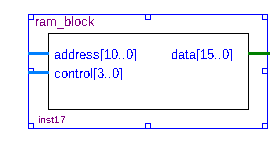
\includegraphics[scale=0.8]{ramb}
    \caption{Блок памяти}
\end{figure}
Блок ram\_block включает в себя синхронные ram и rom, переключение между блоками осуществляется на основе старшего бита адреса.
Временные диаграммы чтения и записи ОЗУ представлены на рисунках 2.1 и 2.2.

Содержимое ROM памяти включает в себя коды команд, записанные последовательно в том порядке, в котором выполняется программа.
Память команд хранится в файле rom.hex.

Блок `ram\_block` содержит 2 входа:
\begin{itemize}
    \item address[10..0] -- адрес ячейки для чтения/записи
    \item control[1..0] -- тактирующий импульс и сигнал режима чтение/запись
\end{itemize}
Двунаправленный вход data[15..0] служит для подключения шины данных.

Содержимое RAM памяти представляет собой данные, которыми оперирует процессор, и в которые происходит запись результатов работы. Содержимое памяти может быть проинициализировано в файле ram.hex.

Синхронная RAM выдает данные на выход на следующем такте, после указания адреса и установления единичного сигнала на входе outenab.

Сигнал inclock на выходах RAM и ROM устанавливается по спаду тактирующего сигнала, outclock -- по фронту.

\subsection{Устройство управления}
Устройство управления устанвливает сигналы, разрешающие работу определенных блоков.
Данный блок представлен в файле 'cu.bdf'.

На вход подается единственный сигнал -- clk. Он служит для тактирования УУ.

\begin{figure}[ht]
\centering
    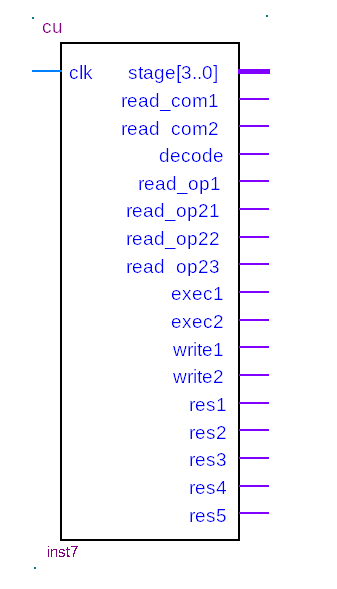
\includegraphics[scale=0.8]{cub}
    \caption{Блок управления}
\end{figure}

Выходы:
\begin{itemize}
    \item stage[3..0] -- отладочный сигнал для наглядного просмотра текущей стадии выполнения команды
    \item read\_com1 -- считывние первого слова команды
    \item read\_com2 -- считывние второго слова команды
    \item decode -- этап декодирования команды
    \item read\_op1 -- чтение первого операнда
    \item read\_op21 -- начало чтения второго операнда
    \item read\_op22 -- запрос в память при косвенной адресации
    \item read\_op23 -- сохранение операнда, полученного из памяти, при косвенной адресации
    \item execute1 -- первый такт операций над операндами
    \item execute2 -- второй такт операций над операндами
    \item write1 -- начало записи результата
    \item write2 -- конец записи результата
    \item res1 - res5 -- резервные выходы
\end{itemize}

\subsection{Блок выборки инструкций}
Данный блок осуществляет выборку инструкций, а также их декодирование.
Блок включает в себя 2 регистра для хранения слов команд, счетчик инструкций.
Схему блока можно найти в файле 'if.bdf'.

\begin{figure}[ht]
\centering
    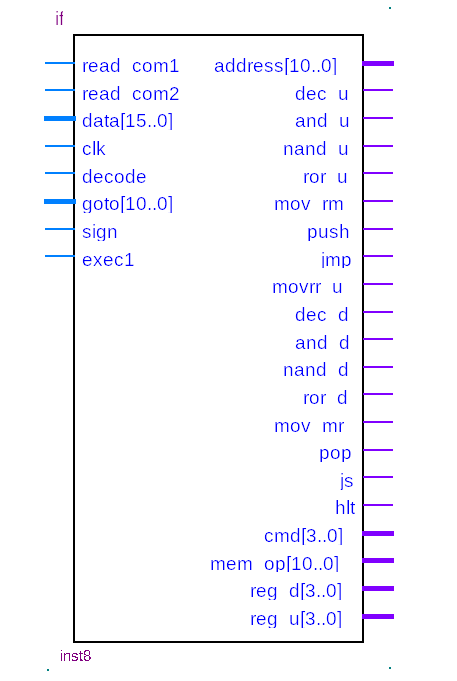
\includegraphics[scale=0.8]{ifc}
    \caption{Блок выборки инструкций}
\end{figure}

Входные сигналы:
\begin{itemize}
    \item clk -- тактирующий сигнал
    \item read\_com1 -- чтение первого слова из памяти
    \item read\_com2 -- чтение второго слова из памяти
    \item decode -- декодирование команды
    \item sign -- флаг знака, служит для операции перехода js
    \item exec1 -- в комбинации с активными сигналами jmp или js и sign приводит к переходу по адресу goto[10..0]
    \item goto[10..0] -- адрес перехода
\end{itemize}
Выходные сигналы:
\begin{itemize}
    \item dec\_d -- декремент. Прямая регистровая адресация
    \item and\_d -- поразрядное И. Прямая регистровая адресация
    \item nand\_d -- поразрядое И-НЕ. Прямая регистровая адресация
    \item ror\_d -- циклический сдвиг вправоИ. Прямая регистровая адресация
    \item dec\_u, and\_u, nand\_u, ror\_u -- аналогичны предыдущим. Косвенная регистровая адресация.
    \item jmp -- безусловный переход
    \item js -- перход при старшем бите равным нулю
    \item hlt -- сигнал выключения микро-ЭВМ
    \item push -- занесение регистра в стек
    \item pop -- чтение регистра из стека
    \item mov\_mr -- пересылка операнда из регистра в память
    \item mov\_rm -- пересылка памяти -> регистр
    \item mov\_rr -- пересылка память -> регистр. Косвенная регистровая адресация
    \item cmd[3..0] -- КОП
    \item mem\_op[10..0] -- адрес операнда, хранящегося в памяти
    \item reg\_d[3..0] -- адрес регистра. Прямая регистровая адресация
    \item reg\_u[3..0] -- адрес регистра. Косвенная регистровая адресация
\end{itemize}

\subsection{Блок выборки операндов}
Осуществляет загрузку операндов из памяти, используя соответсвующую команде адресацию. Блок представлен в файле 'op\_f.bdf'.

\begin{figure}[ht]
\centering
    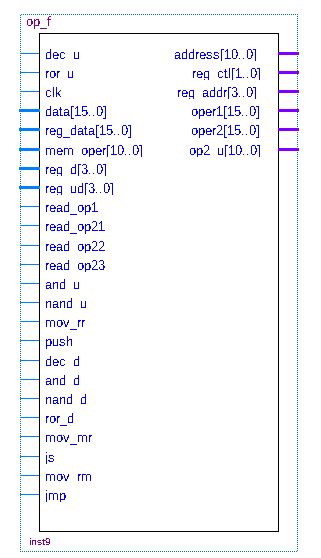
\includegraphics[scale=0.8]{opfb}
    \caption{Блок выборки операндов}
\end{figure}

Входы:
\begin{itemize}
    \item все выходы с предыдущего блока, за исключением hlt, cmd[3..0]
    \item clk -- синхросигнал
    \item reg\_op1 - reg\_op23 -- предоставление процессорного времени
    \item reg\_data[15..0] -- данные из РОН
    \item data[15..0] -- данные из RAM
\end{itemize}
Выходы:
\begin{itemize}
    \item address[10..0] -- адрес для чтения из RAM
    \item reg\_addr[3..0] -- адрес регистра
    \item op1[15..0] -- первый операнд
    \item op2[15..0] -- второй операнд
    \item reg\_ctl[1..0] -- управляющие РОН сигналы
    \item op2\_u[10..0] -- адрес ячейки памяти, при косвенной регистровой адресации
\end{itemize}

\subsection{АЛУ}
Блок АЛУ выполняет арифметические и логические операции, работает со стеком. Если операнды не нуждаются в обработке(например при командах пересылки), АЛУ отправляет их сразу на выход. Также АЛУ содержит регистр, хранящий знак последних выходных данных с АЛУ.

\begin{figure}[ht]
\centering
    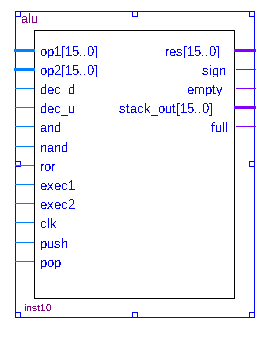
\includegraphics[scale=0.8]{alub}
    \caption{АЛУ}
\end{figure}

Входы:
\begin{itemize}
    \item dec\_d, dec\_u, and, nand, ror, push, pop -- определяют, исполняется ли данная команда сейчас
    \item clk -- синхросигнал
    \item exec1, exec2 -- предоставление процессорного времени
    \item op1[15..0] -- первый операнд
    \item op2[15..0] -- второй операнд
\end{itemize}
Выходы:
\begin{itemize}
    \item res[15..0] -- выходной операнд
    \item stack\_out[15..0] -- данные, выходящие со стека
    \item sign -- флаг установки старшего бита в 1
    \item empty -- стек пуст
    \item full -- стек полон
\end{itemize}

\subsection{Блок сохранения результата}

\begin{figure}[ht]
\centering
    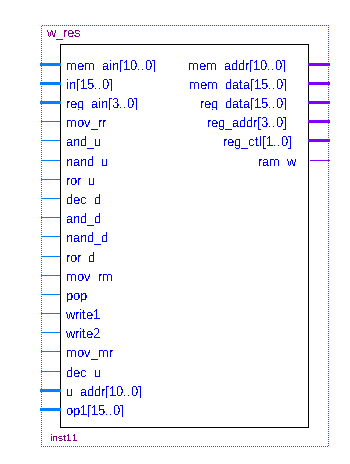
\includegraphics[scale=0.8]{wbc}
    \caption{Блок сохранения результата}
\end{figure}
Входы:
\begin{itemize}
    \item mem\_ain[10..0] -- адрес для записи данных при прямой адресации
    \item in[15..0] -- операнд для записи
    \item u\_addr[10..0] -- адрес для записи операнда при косвенной регистровой адресации
    \item op1[15..0] -- вход для операнда команды dec
    \item write1, write2 -- сигналы разрешения работы
\end{itemize}
Выходы:
\begin{itemize}
    \item ram\_w -- сигнал переключения RAM в режим записи
    \item reg\_ctl[1..0] -- управляющие сигналы РОН
    \item reg\_addr[3..0] -- адрес РОН
    \item reg\_data[15..0] -- данные для записи в РОН
    \item mem\_data[15..0] -- данные для ОЗУ
    \item mem\_addr[10..0] -- адрес памяти для записи операнда
\end{itemize}
Остальные входы -- входы работы соответствующих команд
Блок осуществляет запись операнда в ОЗУ или РОН в зависимости от адресации команды.

\subsection{Блок РОН}
\begin{figure}[ht]
\centering
    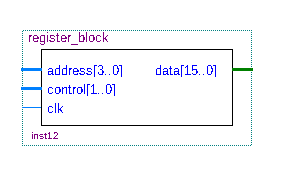
\includegraphics[scale=0.8]{regb}
    \caption{Блок РОН}
\end{figure}

Входы:
\begin{itemize}
    \item address[3..0] -- адрес регистра
    \item control[1..0] -- управляющий вход
    \item clk -- синхросигнал
\end{itemize}
Двунапраленные порты:
\begin{itemize}
    \item data[15..0] -- данные
\end{itemize}

Блок РОН содержит 10 шестнадцатиразрядных регистров общего назначения. Регистры могут хранить как данные, так и адреса ячеек памяти.

\subsection{Стек}
Содержит 11 шестнадцатиразрядных регистров. Позволяет работать с регистрами по принципу FIFO. На схеме блок имеет название 'Stack'.

\begin{figure}[ht]
\centering
    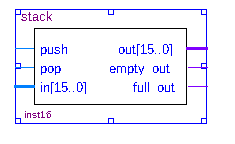
\includegraphics[scale=0.8]{stackb}
    \caption{Стек}
\end{figure}

Входы:
\begin{itemize}
    \item push -- запись регистра в стек
    \item pop -- освобождение регистра из стека
    \item in[15..0] -- входной регистр
\end{itemize}
Выходы:
\begin{itemize}
    \item out[15..0] -- выходной регистр
    \item empty -- стек пуст
    \item full -- стек полон
\end{itemize}
Стек растет вверх, указатель стека указывает на следующую свободную ячейку.
При включении сигнала full -- запись в стек блокируется, при активном сигнале empty -- отсутствует запись операнда команды pop на шаге сохранения операндов.


%
%
\newcommand{\companyname}{\mbox{<<Техартгруп>>}}

\section{Охрана труда}

\subsection[Обеспечение пожарной безопасности на предприятии]{Обеспечение пожарной безопасности на предприятии малого бизнеса \companyname{}}


Целью дипломного проекта является реализация и анализ алгоритмов построения вероятностных сетей.
Вероятностная сеть является компактным и эффективным способом представления знаний.
Вероятностные сети используются в программном обеспечении для принятия решения в условиях недостаточной определенности.
Данный способ статистического моделирования показал свою пригодность в реальных условиях в сложных предметных областях: медицине, космической промышленности, финансовой сфере и других областях.
Первоначальные стадии разработки дипломного проекта выполнялись на предприятии ООО~\companyname{} во время прохождения преддипломной практики.
В настоящем разделе рассматриваются вопросы, связанные с обеспечением пожарной безопасности на предприятии.

Предприятие \companyname{} занимается предоставлением услуг по разработке информационных систем для иностранных предприятий.
В минском офисе компании на данный момент работает более 200 человек.
% TODO: Переписать абсолютный бред в оставшейся части абзаца.
Большое количество конкурирующих компаний, разрабатывающих программное обеспечение в Минске, способствует повышению общего уровня условий труда.
Это, в частности, сказывается на комфортабельности рабочих мест.
Работникам предоставляются светлые, проветриваемые, тихие кабинеты, гибкий график рабочего времени, специальные комнаты отдыха и т.\,д.
Современные компании негласно ориентируются на соответствие лучшим мировым практикам в области охраны труда и, в частности, пожарной безопасности.

На предприятии \companyname{} за пожарную безопасность отвечает директор компании.
Для каждого нового сотрудника производится инструктаж по пожарной безопасности и технике безопасности, а так же знакомство с планом эвакуации при возникновении черезвычайных ситуаций~\cite[\ignore{раздел~5.5.8,} с.~324]{michnuk_2009}.
За проведение инструктажа отвечает специальный человек из отдела материально"=технического снабжения предприятия.
В компании действует набор правил, обязательных для исполнения сотрудниками.
В целях повышения пожарной безопасности курение в здании офиса запрещено.
Все сотрудники обязаны в конце рабочего дня выключить свои персональные компьютеры и обесточить их.
В конце рабочего дня специальный сотрудник проверяет соблюдение данного правила в каждом рабочем кабинете, чтобы там были выключены все электрические приборы: компьютеры, электрические чайники, кондиционеры, освещение и т.\,д.
Все рабочие компьютеры подключены к источникам бесперебойного питания, которые подключены к сетевыми фильтрам, защищающим от скачков напряжения в электросети.

Офис компании расположен в центре города.
Здание офиса представляет собой монолитную железобетонную конструкцию высотой шесть этажей, офис компании находится на двух верхних этажах.
Конструкция здания предусматривает три способа эвакуации с этажа: выход в паркинг, лестничная клетка с выходом на улицу, лестничная клетка с выходом на первый этаж паркинга.
В случае недоступности основных эвакуационных выходов из каждого кабинета можно через окно попасть на лоджию~\cite[\ignore{раздел~5.5.4,} с.~314\,--\,316]{michnuk_2009}.
Схемы эвакуации выдаются в виде электронного документа каждому новому сотруднику, а также находятся на специальном стенде в рабочих кабинетах.
Все кабинеты офиса расположены вдоль длинного коридора, который оборудован специальными аварийными светильниками и знаками, указывающими направление эвакуации.
На случай отключения электроэнергии компания имеет два дизельных"=генератора, обеспечивающих нужды предприятия на случай отключения электроэнергии.

Офис компании оборудован необходимыми средствами сигнализации о пожаре~\cite[с.~215]{sinilov_2010}. %\cite[с.~5\,--\,7]{sharovar_1979}.
Каждый кабинет оборудован пожарным дымовым оптико"=электрическим точечным извещателем \mbox{ИП212-02М1} (рисунок~\ref{fig:fire_alarms}).
На предприятии производиться регулярный контроль и проверка работоспособности пожарных извещателей специальным человеком из отдела материально"=технического снабжения предприятия.
В коридорах дополнительно установлены ручные пожарные извещатели \mbox{ИП 5-2Р} (рисунок~\ref{fig:fire_alarms}).
Для извещения о пожаре также может быть использована корпоративная электронная почта, а также другие современные способы обмена информацией.

\begin{figure}[ht]
\centering
  \begin{subfigure}[b]{0.45\textwidth}
    \centering
    \includegraphics[scale=0.85]{avt_pozh_izv.jpg}
    \caption{}
  \end{subfigure}
  \begin{subfigure}[b]{0.45\textwidth}
    \centering
    \includegraphics[scale=1.2]{ruch_pozh_izv.jpg}
    \caption{}
  \end{subfigure}
  \caption{ а "--- автономный пожарный извещатель;
            б "--- ручной пожарный извещатель.}
  \label{fig:fire_alarms}
\end{figure}

На случай возникновения пожара в каждом рабочем кабинете находиться ручной порошковый огнетушитель \mbox{ОП-10}~(з)~МИГ~М (рисунок~\ref{fig:extinguishing_fire}), пригодный для тушения пожаров различного типа, в том числе для тушения электрических приборов~\cite[\ignore{раздел 5.5.7,} с.~221\,--\,323]{michnuk_2009}.
Каждый этаж здания офиса оборудован двумя пожарными кранами для тушения пожара.
Пожарные краны расположены в противоположных частях коридора, недалеко от эвакуационных выходов (рисунок~\ref{fig:extinguishing_fire}).
На случай воспламенения электрической проводки или другого электрического оборудования в каждом кабинете установлены электрические щитки, необходимые для отключения подачи электроэнергии в пределах кабинета.
Во всех помещениях офиса предприятия установлена оросительная система пожаротушения для ликвидации возгорания до приезда пожарной службы~\cite[\ignore{раздел~5.5.6,} с.~318\,--\,320]{michnuk_2009}.
При расследовании возможных причин возникновения пожара может быть задействована система видео"=наблюдения, установленная во всех помещениях предприятия.

\begin{figure}[ht]
\centering
  \begin{subfigure}[b]{0.45\textwidth}
    \centering
    \includegraphics[scale=0.34]{ognetush.jpg}
    \caption{}
  \end{subfigure}
  \begin{subfigure}[b]{0.45\textwidth}
    \centering
    \includegraphics[scale=0.7]{pozh_kran.jpg}
    \caption{}
  \end{subfigure}
  \caption{ а "--- порошковый огнетушитель \mbox{ОП-10}~(з)~МИГ~М;
            б "--- пожарный кран.}
  \label{fig:extinguishing_fire}
\end{figure}

Основной род деятельности на предприятии "--- разработка информационных систем "--- не предусматривает непосредственный контакт с горючими или легко"=воспламеняющимися веществами, что сильно снижает риски возникновения пожара на предприятии.
Наиболее вероятными причинами возникновения пожара, с учетом специфики предприятия, могут являться нарушение правил внутреннего распорядка "--- курение на рабочем месте, и неисправность электрического оборудования, которого в офисе компании достаточно~\cite[\ignore{раздел 5.5.1,} с.~312]{michnuk_2009}.
С целью снижения риска возникновения пожара по причине неисправности электрического оборудования в компании запрещено пользоваться неисправным оборудованием, а все исправное оборудование подключается в сеть через специальные сетевые фильтры и источники бесперебойного питания.
В целом правила распорядка на предприятии и высокая культура работы с электрическим оборудованием снижают риски возникновения пожара до минимума.

Большой проблемой в достижении максимальной пожарной безопасности предприятия является доступность подъезда пожарной техники к зданию офиса.
В будние дни прилегающие улицы, стоянки, пешеходные переходы заняты неправильно припаркованным личным транспортом.
Большую часть светлого времени суток движение по прилегающим улицам очень затруднено.
Данную проблему предприятие не в силах решить самостоятельно, проблема заключается в низкой культуре владельцев транспорта и игнорировании многочисленных нарушений правил дорожного движения  сотрудниками ГАИ.
% Заключительное предложение
Таким образом, изложенные выше предложения, не смотря на проблемы с подъездом пожарной техники, обеспечат пожарную безопасность на предприятии \companyname{}.

%
% \include{sec_econ}
\section{Анализ и оптимизация разработанной микро-ЭВМ}
Для оптимизации работы системы, улучшения масштабируемости и модульности при разработке микро-ЭВМ применялись различные приемы:

    \begin{itemize}
        \item Все команды имеют одинаковую длину, это позволяет упростить схему, тем самым снижая ее стоимость.
        \item Все операнды в команде занимают фиксированные адреса, тем самым сильно упрощается выборка команд. Добавление новых команд также не вызовет особых сложностей.
        \item Все стадии исполнения команды занимают фиксированное количество тактов -- упрощается логика устройства управления.
        \item Адреса памяти при прямой адресации располагаются в младших битах слова. Это позволяет облегчить отладку схемы.
        \item Простое строение адресного пространство памяти. Старший бит адреса определяет, какому устройству принадлежит адрес. Тем самым снижаются затраты на определение принадлежности адреса, но также это приводит к тому, что на ROM отводится половина всего адресного пространства.
    \end{itemize}

	Из недостатков системы можно указать следующие:
    \begin{itemize}
        \item Отсутствие кэша. При обращении к памяти теряется большое количество тактов. Это особенно большая проблема в Принстонской архитектуре, потому что данные и инструкции передаются через одну шину, тем самым сильно снижая производительность системы.
        \item Отсутствие контроллера прямого доступа к памяти. В случае необходимости передачи данных между каким-нибудь внешним источником и памятью необходимо затрачивать процессорное время.
        \item Отсутствует конвейеризация. Наличие конвейера позволило бы уменьшить среднее время выполнения одной команды.
        \item Отсутствие арбитража шин. Нету единой схемы доступа к устройствам, в результате чего происходит дублирование компонентов и увеличение сложности схемы.
    \end{itemize}


%
\include{sec_final}
% Зачем: Изменение надписи для списка литературы
% Почему: Пункт 2.8.1 Требований по оформлению пояснительной записки.
% \renewcommand{\bibsection}{\sectioncentered*{Cписок использованных источников}}
% \phantomsection\pagebreak% исправляет нумерацию в документе и исправляет гиперссылки в pdf
\sectioncentered*{список использованных источников}
\addcontentsline{toc}{section}{Список использованных источников}
% \addcontentsline{toc}{section}{Cписок использованных источников}

% Зачем: Печать списка литературы. База данных литературы - файл bibliography_database.bib

1. Столлингс, У. Структурная организация и архитектура компьютерных
систем/ У. Столлингс. 5-е изд. – М.: "Вильямс", 2001. Пер. с англ. – 892 с.

2. Таненбаум, Э. Архитектура компьютерных систем/ Э. Таненбаум. 4-е
изд. – М.: "ПИТЕР", 2002. Пер. с англ. – 698 с.

3. Цилькер, Б.Я. Организация ЭВМ и систем/ Б.Я. Цилькер, С.А. Орлов. –
М.: "Питер", 200. – 668 с.

4. Грушвицкий, Р. Проектирование систем на микросхемах программируемой логики/ Р. Грушвицкий. – СПб.: "Питер", 2002. – 608 с.

5. Угрюмов Е. Цифровая схемотехника. - М.: "С-Петербург", 2001, 518 стр.

6. Майоров С.А. Введение в микроЭВМ. - Л.: Машиностроение, 1988.

7. Солонина А. Алгоритмы и процессоры цифровой обработки сигналов. -
СПб.: "Питер", 2001. – 464 с.

8. Шагурин И.И. Процессоры семейства Intel Р6. Архитектура, программирование, интерфейс. – М.: "Телеком", 2000. – 248 с.

9. Рудометов Е. Материнские платы и чипсеты. – СПб.: "Питер", 2000. –
256 с.

10. Бибило П.Н. Синтез логических схем с использованием языка VHDL.
М.: СОЛОН-Р, 2002.

11. Антонов А. П. Язык описания цифровых устройств AlteraHDL. - М. :
РадиоСофт, 2001.

12. Глецевич И.И., Прытков В.А., Отвагин А.В. Методические указания по
дипломному проектированию для студентов специальности 40 02 01 «Вычис-
лительные машины, системы и сети». – Минск БГУИР, 2009, 99 с.
% \bibliography{bibliography_database}


% %
% % Зачем: Изменение надписи для списка литературы
% Почему: Пункт 2.8.1 Требований по оформлению пояснительной записки.
% \renewcommand{\bibsection}{\sectioncentered*{Cписок использованных источников}}
% \phantomsection\pagebreak% исправляет нумерацию в документе и исправляет гиперссылки в pdf
\sectioncentered*{список использованных источников}
\addcontentsline{toc}{section}{Список использованных источников}
% \addcontentsline{toc}{section}{Cписок использованных источников}

% Зачем: Печать списка литературы. База данных литературы - файл bibliography_database.bib

1. Столлингс, У. Структурная организация и архитектура компьютерных
систем/ У. Столлингс. 5-е изд. – М.: "Вильямс", 2001. Пер. с англ. – 892 с.

2. Таненбаум, Э. Архитектура компьютерных систем/ Э. Таненбаум. 4-е
изд. – М.: "ПИТЕР", 2002. Пер. с англ. – 698 с.

3. Цилькер, Б.Я. Организация ЭВМ и систем/ Б.Я. Цилькер, С.А. Орлов. –
М.: "Питер", 200. – 668 с.

4. Грушвицкий, Р. Проектирование систем на микросхемах программируемой логики/ Р. Грушвицкий. – СПб.: "Питер", 2002. – 608 с.

5. Угрюмов Е. Цифровая схемотехника. - М.: "С-Петербург", 2001, 518 стр.

6. Майоров С.А. Введение в микроЭВМ. - Л.: Машиностроение, 1988.

7. Солонина А. Алгоритмы и процессоры цифровой обработки сигналов. -
СПб.: "Питер", 2001. – 464 с.

8. Шагурин И.И. Процессоры семейства Intel Р6. Архитектура, программирование, интерфейс. – М.: "Телеком", 2000. – 248 с.

9. Рудометов Е. Материнские платы и чипсеты. – СПб.: "Питер", 2000. –
256 с.

10. Бибило П.Н. Синтез логических схем с использованием языка VHDL.
М.: СОЛОН-Р, 2002.

11. Антонов А. П. Язык описания цифровых устройств AlteraHDL. - М. :
РадиоСофт, 2001.

12. Глецевич И.И., Прытков В.А., Отвагин А.В. Методические указания по
дипломному проектированию для студентов специальности 40 02 01 «Вычис-
лительные машины, системы и сети». – Минск БГУИР, 2009, 99 с.
% \bibliography{bibliography_database}


% \includepdf позволяет включить в результирующий pdf документ часть другого pdf документа, сделанного
% например не с помощью TeX. Бывает полезно, если какие-то диаграммны нарисованы, например, с помощью
% Microoft Office и сохранены в pdf.
%\includepdf[pages={-}]{documents_list.pdf}

\end{document}
